\subsection{Fonction chromatique $P_G(k)$}
Le nombre de manières de colorier un graphe est le produit des nombres de façons de colorier chaque sommet.
\begin{itemize}
\item Si le graphe $G$ est complet, nous aurons $k$ couleurs possibles pour le premier sommet, $(k-1)$ pour le deuxième, etc\ldots (Le graphe G étant complet, la couleur du premier sommet est nécessairement exclu des autres sommets).

Le $n$-ième sommet pourra être colorié de $k-(n-1)$ manières. D'où :
\[ P_{K_n}(k)=\prod_{i=0}^{n-1}(k-i) \]

\item Si $G$ est vide, la coloration d'un sommet ne contraint pas la coloration des autres sommets. Nous obtenons alors :
\[ P_{\overline{K_n}}(k)=k^n \]
\end{itemize}

\subsection{Nombre chromatique $\chi(G)$}
Nous appelons \og nombre chromatique \fg de $G$ : $\chi(G)$ étant, par définition, le nombre minimum de couleurs nécessaires pour colorier $G$. Si $k < \chi(G)$ alors le graphe $G$ ne peut pas être colorié par $k$ couleurs. Si $k \geq \chi(G)$ alors il doit y avoir au moins une manière de colorier $G$, celui utilisant $\chi(G)$ couleurs.

Nous avons donc :
\begin{displaymath}
	P_G(k) \left\{ \begin{array}{ll}
	=0 & \textrm{si $k < \chi(G)$} \\
	\geq 1 & \textrm{sinon}
	\end{array} \right.
\end{displaymath}

\subsection{Décomposition de $P_G$}
Montrons d'abord que la propriété est vraie pour tout graphe complet $K_n$. Pour commencer nous remarquons que pour tout arrête $e$:

\begin{itemize}
\item $K_{n\backslash e}$ est exactement $K_{n-1}$, et donc: 

\[ P_{K_n\backslash e}(k) = P_{K_{n-1}} = \prod_{i=0}^{n-2}(k-i) \]


\item Soit $e = (a,b)$. Sans perte de généralité, nous pouvons supposer que $b$ est considéré en dernier lors de la coloration de $K_n$, donc qu'il lui reste $k-(n-1)$ couleurs. Pour colorier $K_{n-e}$ nous aurons un choix de plus pour lui, à savoir la couleur de $a$, donc $k-(n-2)$ en totale. 

De ce fait:

\[ P_{K_n-e}(k) = P_{K_{n-1}}(k)(k-(n-2)) = (\prod_{i=0}^{n-2}(k-i))(k-(n-2)) \]
\end{itemize}

Nous avons donc très clairement:
\begin{eqnarray*}
P_{K_n-e}(k) -  P_{K_n\backslash e}(k) &=& (\prod_{i=0}^{n-2}(k-i))(k-(n-2)) - \prod_{i=0}^{n-2}(k-i)\\
&=& \prod_{i=0}^{n-2}(k-i)(k-(n-1))\\
&=& \prod_{i=0}^{n-1}(k-i)\\
&=& P_{K_n}(k)
\end{eqnarray*}
Tout graphe de rang $n$ peut se générer à partir de $K_n$ (en enlevant des arrêtes). Nous admettrons que la suppression d'arête conserve notre propriété, donc que pour tout graphe $G$ et tout arrête $a$ de celui-ci ($a$ et $e$ sont supposées distinctes):

\begin{eqnarray*}
&&P_G(k) = P_{G-e}(k) - P_{G \backslash e}(k) \\
&\Rightarrow&  P_{G-a}(k) = P_{G-e-a}(k) - P_{G \backslash e-a}(k)
\end{eqnarray*}

Par induction structurelle nous avons donc $P_G(k) = P_{G-e}(k) - P_{G \backslash e}(k)$ pour tout graphe $G$.

\subsection{Polynôme chromatique ?}
Soit $H$ un prédicat tel que :
\begin{displaymath}
	H(m) = \left\{ \begin{array}{ll}
	\top & \textrm{si $\forall$ $G$, graphe de $m$ arrêtes ou moins, $P_G(k)$ est polynomiale.} \\
	\bot & \textrm{sinon.}
	\end{array} \right.
\end{displaymath} 
\begin{itemize} 
\item Nous rappelons que $P_{\overline{K_n}}(k)=k^n$, donc $H(0)$ est vraie. 
\item Supposons $\exists m \in \mathbb{N}$ $|$ $H(m)$ l'est également. Ajoutons l'arc $a$ à $G$. $G_{m+e}$ est un graphe à $(m+1)$ arêtes :

\[ P_{G_{m+z}} = P_{G_{m+e}-e} - P_{G_{m+e} \backslash e} \]

Clairement $P_{G_{m+1}-e}$ et $P_{G_{m+1} \backslash e}$ ont $(m+1)-1 = m$ arêtes. Or par hypothèse de récurrence $H(m)$ est vraie,
$P_{G_{m+1}}$ est la différence entre deux polynômes, donc il est également polynomiale. Nous avons donc $H(m+1)$.
\item Nous venons de montrer $(H(0) \wedge (H(m) \Rightarrow H(m+1)))$. Par récurrence nous avons donc $H(m)$ vrai $\forall m \in \mathbb{N}$. 

\end{itemize} 

\subsection{Application de la décomposition}
Utilisons la formule trouvée au point précédent, et admettons que pour $P_n$ la chaîne de taille $n$ nous avons :
\[ P_{P_n}(k) = k(k-1)^{n-1} \]

Prenons $A$ le graphe initial :
\begin{eqnarray*}
P_A(k) & = & P_B(k) - P_C(k) \\
&=& \big(P_D(k)-P_E(k)\big)-\big(P_F(k)-P_{P_3}(k)\big)\\
&=& \Big[\big(P_{P_5}(k)-P_{P_4}(k)\big)-\big(P_{P_4}(k)-P_{P_3}(k)\big)\Big]-\Big[\big(P_{P_4}(k)-P_{K_3}(k)\big)-P_{P_3}(k)\Big]\\
&=& P_{P_5}(k)+2P_{P_3}(k)-P_{K_3}(k)+3P_{P_4}(k)\\
&=& k(k-1)^4 +2k(k-1)^2+k(k-1)(k-2)-3(k-1)^3 \\
&=& k(k-1)\big[(k-1)^3+z(k-1)+(k-z)-3(k-1)^2\big]\\
&=& (k^2-k)\Big[(k-1)^2\big((k-1)-3\big)+3k -4 \Big]\\
&=& (k^2-k)[k^3-6k^2+12k-8]\\
&=& k^5-7k^4+18k^3-20k^3+8k
\end{eqnarray*}
Où :

$A$ : \raisebox{-0.5\height}{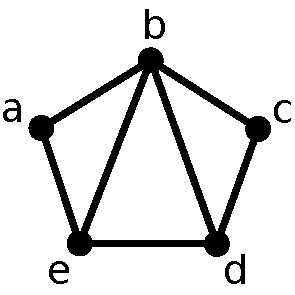
\includegraphics[width=2cm]{files/gAex1.pdf}}

\begin{tabular}{llcll}
$B = A-(e,d) $ : & \raisebox{-0.5\height}{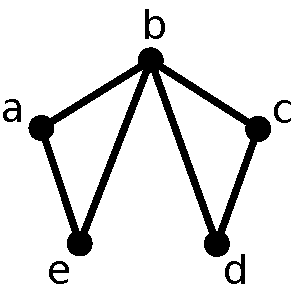
\includegraphics[width=2cm]{files/gBex1.pdf}} & et & $C = A\backslash(e,d)$ : & \raisebox{-0.5\height}{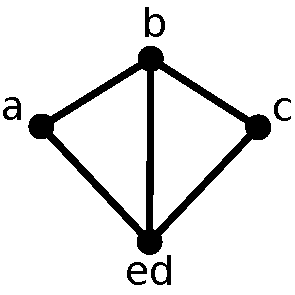
\includegraphics[width=2cm]{files/gCex1.pdf}} \\
$D = C-(a,b)$ : & \raisebox{-0.5\height}{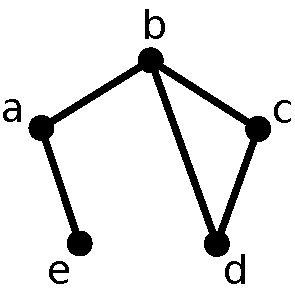
\includegraphics[width=2cm]{files/gDex1.pdf}} & et & $E = C\backslash(e,b)$ : & \raisebox{-0.5\height}{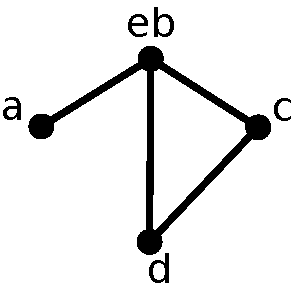
\includegraphics[width=2cm]{files/gEex1.pdf}} \\
$F = C-(b,ed)$ : & \raisebox{-0.5\height}{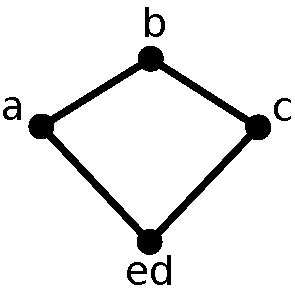
\includegraphics[width=2cm]{files/gFex1.pdf}}& et & $C \backslash(b,ed) = P_3$ : & \raisebox{-0.5\height}{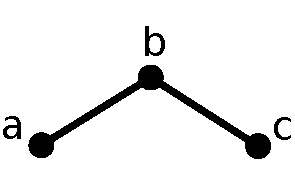
\includegraphics[width=2cm]{files/gC-ex1.pdf}}
\end{tabular}

\subsection{Particularités des polynômes chromatiques}
Nous cherchions à prouver que pour tout graphe $G$ à $n$ sommets et $m$ arrêtes, avec $C = \{c_i\}$ un ensemble de coefficients naturels (donc positifs) : 
\[ P_G(k) = k^n - mk^{n-1} + \sum_{i = 2}^n \Big((-1)^i(c_ik^{n-i})\Big) \]
Nous nommerons $F_k(n,m,C)$ cette forme polynomiale particulière. Soit $H$ un prédicat tel que :
\[ H(n,m) \Leftrightarrow \forall{G(n,m)}, \hspace{1mm} \exists{C} \hspace{1mm} 
										| \hspace{1mm} P_G(k) = F(n, m, C) \]
Nous montrerons par récurrence que $H(n,m)$ est vrai pour tout $n$ et tout $m$ :
\begin{itemize}
\item \textbf{Sommets -- cas de base} \\
Pour $n = 1$ nous avons $P_G(k) = k$, donc $H(1,0)$ est vérifié.
\item \textbf{Sommets -- pas récursif} \\ Supposons qu'il existe un nombre de sommets $n_0$ et un nombre d'arêtes $m_0$ tel que $H(n_0,m_0)$ soit vrai. Soit $G$ un graphe à $n_0$ sommets et $m_0$ arêtes, et $G^+$ le graphe généré en reliant un nouveau sommet $s'$ à une sélection de $n' \leq n_0$ sommets de $G$. Nous aurons donc $(k-n')$ manières de colorier $s'$.

De ce fait:
\[ P_{G^+}(k) = P_G(k)(k-n') \]
Où $P_G(k)$ est de la forme $F$. $P_G^+(k)$ est donc de la forme:
\begin{eqnarray*}
&&	F(n,m,C)(k-n')			\\
&=& F(n,m,C)k - n'F(n,m,C)	
\end{eqnarray*} 
\begin{itemize}
\item \textbf{Maintient des signes alternatifs} \\ 
Le fait de multiplier par $k$ \og décale \fg les termes du polynôme à gauche. Soustraire $n'F_k(n,m,C)$ retranche alors au coefficient de chaque terme $n'$ fois celui de leur voisin de gauche, avec $0 \leq n' \leq n$. Or si le terme est positif, son voisin de gauche est négative par hypothèse, donc son coefficient augmentera.

De même si le terme est négative son coefficient va diminuer. Les signes resteront donc alternatifs dans $P_G^+(k)$.

\item \textbf{Maintient de $k^n$} \\
$k^{n}$ deviendra $k^{n+1}$ dans $F_k(n,m,C)k$ et, n'aillant pas de voisin gauche dans $F_k(n,m,C)$, nous ne lui retrancherons rien. La propriété sur le terme de plus haut degré est donc maintenu.

\item \textbf{Maintient de $mk^{n-1}$} \\
Le terme $-mk^{n-1}$, aillant pour voisin gauche $k^n$, deviendra
\[-mk^n - n'k^n = -(m+n')k^n \]
$(m+n')$ étant le nombre d'arêtes de $G^+$. La propriété sur le second terme de plus haut degré est alors maintenu aussi.
\end{itemize}
Nous avons donc $H(n_0+1, m_0)$, qui nous servira pas la suite\ldots

\item \textbf{Arrêtes -- cas de base} \\
Pour $m = 0$ nous avons $G = \overline{K}_n$ et donc $P_G(k) = P_{\overline{K}_n}(k) = k^n$. Du coup $\forall n \in \mathbb{N^+}$, $H(n,0)$ est vrai.

\item \textbf{Arrêtes -- pas récursive} \\
Supposons qu'il existe un nombre d'arêtes $m_0$ tel que pour tout $m \leq m_0$ et tout $n$ nous avons $H(n,m_0)$. Soit $G$ un graphe à $n$ sommets et $m_0 + 1$ arrêtes. D'après la formule de la question 3, nous avons :
\begin{eqnarray*}
P_G(k) &=& P_{G-e}(k) - P_{G \backslash e}(k)	\\
		&=& F_k(n,m_0,C') - F_k(n-1,m_0+1-n',C'')	\\
		&=& \Big( k^n - m_0k^{n-1} + \ldots \Big) - \Big( k^{n-1} - (m_0+1-n')k^{n-2} + \ldots \Big) 	\\
		&=& k^n - (m_0+1)k^{n-1} + \ldots	\\
		&=& F_k(n, m_0+1, C''')									
\end{eqnarray*}

Nous admettons ci-dessus la conservation de alternance des signes. De ce fait nous avons $H(n,m_0+1)$.
\end {itemize}
Nous avions démontrés précédemment :
\[ H(1,0) \wedge H(n,0) \wedge (H(n,m) \Rightarrow H(n+1,m)) \wedge (H(n,m \Rightarrow H(n,m+1)) \]
Par récurrence nous avons donc $H(n,m)$ pour tout pair $(n,m)$ de $\mathbb{N}^*\times{\mathbb{N}}$

\subsection{Polynôme chromatique de $K_{1,5}$}
$K_{1,5}$ étant un arbre, nous aurons $k$ choix de coloration pour la racine, peu importe le choix de celle-ci, et $k-1$ pour les autres, car chaque sommet considéré sera relié à exactement une autre déjà colorié. Au final, nous avons donc:
\begin{eqnarray*}
P_{K_{1,5}}(k) 	& = & k(k-1)^5 \\
				& = & k{((k-1)^2)}^2(k-1)	\\
				& = & k(k^2 - (2k - 1))^2(k-1)	\\
				& = & (k^5 - 4k^4  + 6k^3 - 4k^2 + k)(k-1)  \\
				& = & k^6 - 5k^5  + 10k^4 - 10k^3 + 5k^2 - k	 
\end{eqnarray*}

\subsection{Coloration de graphes non-connexes}
La coloration de chaque composante connexe $C_i$ n’influe pas sur celle des autres. Du coup le nombre de manières de colorier un graphe entier est le produit des polynômes chromatiques de ses composantes connexes:
\begin{eqnarray*}
G = \bigcup_{i=0}^n C_i & \Rightarrow & P_G(k)=\prod_{i=0}^n P_{C_i}(k) \\
\end{eqnarray*}

\subsection{Coloration d'arbres}
Supposons que nous ayons un graphe $G$ tel que $P_G(k) = k(k-1)^{n-1}$ :
\begin {itemize}
\item Intuitivement cela signifie que nous avons $k$ choix de couleurs pour le premier sommet colorié, puis $(k-1)$ pour chacun des $(n-1)$ autres. Chaque sommet, lors de sa coloration, ne doit être en contact qu'avec un seul sommet déjà colorié. Ceci n'est possible que dans un graphe sans cycle, car même avec un seul cycle nous aurons au plus $k(k-1)^{n-2}(k-2) < k(k-1)^{n-1}$ colorations différentes.
\item De même si $G$ est une forêt, même si elle n'est composé que de deux composantes connexes, il devraient y avoir au moins $k^2(k-1)^{n-2} > k(k-1)^{n-1}$ colorations possibles.
\end {itemize}
Nous avons donc $G$ connexe et sans cycle: il s'agit de la définition même d'un arbre.

\subsection{Trois graphes}
Grâce aux développements précédents (questions 7 et 12) nous reconnaissons :
\begin{eqnarray*}
&&		k^5 - 4k^4 + 6k^3 - 4k^2 + k 	\\	
&=&		k(k-1)^4						\\
&=&		P_{P_5}(k)						
\end{eqnarray*}
Notre premier exemple sera donc $P_5$ le chemin de taille $5$. Or, d'après la propriété de la question 6, nous ne cherchons ici que des graphes aillant 5 sommets et 4 arrêtes. De plus, d'après la propriété de la question 9, ils doivent être des arbres. Nous prenons donc le graphe étoile $S_5 = K_{1,4}$ ainsi que l'arbre à 5 sommets dont la particularité est d'être sans particularité (que nous nommerons $A_5$) :

\begin{center}
$P_5$ : \raisebox{-0.5\height}{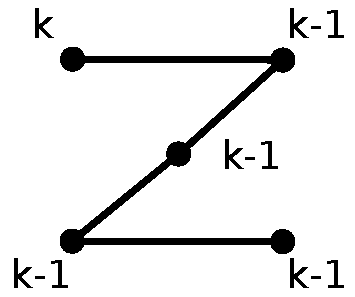
\includegraphics[width=2cm]{files/p5ex1.pdf}} \hspace{1cm}
$S_5$ : \raisebox{-0.5\height}{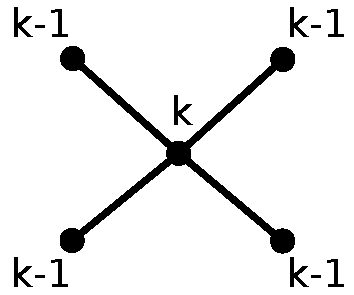
\includegraphics[width=2cm]{files/s5ex1.pdf}} \hspace{1cm}
$A_5$ : \raisebox{-0.5\height}{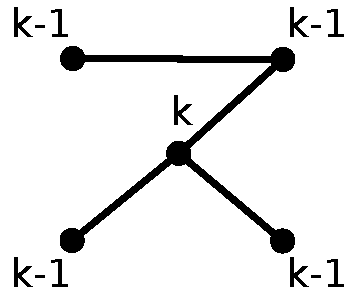
\includegraphics[width=2cm]{files/a5ex1.pdf}}
\end{center}

\subsection{Polynôme chromatique de $K_{2,5}$}
Nous avions déjà calculé le polynôme chromatique de $K_{1,5}$ :
\[ P_{K_{1,5}}(k) = k^6 - 5k^5  + 10k^4 - 10k^3 + 5k^2 - k \]
Or $K_{2,5}$ se construit à partir de $K_{1,5}$ par l'ajout d'un sommet relié au 5 sommets de la partition majoritaire. Ce nouveau sommet pourra être colorié de $(k-5)$ manières, car seront interdits les couleurs de ses 5 voisins. Nous avons donc :
\begin{eqnarray*}
P_{K_{2,5}} & = &	(P_{K_{1,5}}(k))(k-5)								\\
			& = & 	(k^6 - 5k^5  + 10k^4 - 10k^3 + 5k^2 - k)(k-5)		\\	
			& = &	k^7 - 10k^6 + 35k^5 - 60k^4 + 55k^3 - 26k^2 + 5k	
\end{eqnarray*}

\subsection{Polynômes chromatiques de $C_4$ et $C_5$}
\begin {itemize}
\item Pour calculer $P_{C_4}$, commençons par constater que $C_3 = K_3$ :
\begin{eqnarray*}
P_{C_4}(k)	& = &	P_{P_4}(k) - P_{K_3}(k)				\\
			& = & 	k(k-1)^3 - k(k-1)(k-2)				\\
			& = & 	(k^2 - k)((k-1)^2 - (k-2))			\\
			& = &	(k^2 - k)(k^2 - 3k + 3)				\\
			& = & 	k^4 - 4k^3 + 6k^2 - 3k							
\end{eqnarray*}
\item Nous pouvons alors utiliser $P_{C_4}$ pour calculer $P_{C_5}$ :
\begin{eqnarray*}
P_{C_5}(k)	& = &	P_{P_5}(k) - P_{C_4}(k)				\\
			& = & 	k(k-1)^4 - k^4 -4k^3 + 6k^2 - 3k	\\
			& = &	k^5 - 5k^4 + 10k^3 - 10k^2 + 4k		 
\end{eqnarray*}
\end {itemize}

\subsection{Coloration de cycles}
Soit $H$ un prédicat tel que : 
\[ H(n) \Leftrightarrow \Big(P_{C_n}(k) = \big((k-1)^n + (-1)^n(k-1)\big)\Big) \]
\begin{itemize}
\item Prenons comme cas de base $n = 3$ :
\begin{eqnarray*}
P_{C_3}(k) 				& = &	P_{K_3}(k)						\\ 
						& = &	k(k-1)(k-2)						\\
						& = &	k^3 - 3k^2 + 2k					\\
						& = &   k^3 - 3k^2 + 3k - 1 - k + 1 	\\
						& = &	(k^2 -2k + 1)(k-1) - (k-1)		\\
						& = &	(k-1)^3 -(k-1) 					
\end{eqnarray*} $H(3)$ est donc vrai.
\item Supposons $H(n)$ vrai pour un $n$ donnée. Suivant cette hypothèse nous avons :
\begin{eqnarray*}
P_{C_{n+1}}(k)			& = & P_{C_{n+1}-e} - P_{C_{n+1}\backslash{e}}(k)	\\
						& = & P_{P_{n+1}}(k) - P_{C_n}(k)					\\
						& = & k(k-1)^n - \Big((k-1)^n + (-1)^n(k-1)\Big)	\\
						& = & (k-1)(k-1)^n - (-1)^n(k-1)					\\
						& = & (k-1)^{n+1} (-1)^{n+1}(k-1)					
\end{eqnarray*}
Nous avons donc $H(n+1)$.
\end{itemize}
En conclusion : $H(3) \wedge (H(n) \Rightarrow H(n+1))$. Par récurrence nous avons donc $H(n)$ vrai pour tout $n \geq 3$. 
(À noter qu'on ne rencontre pas souvent de cycles de taille inférieur à 3.)

\subsection{Coloration de graphes bipartis complets}
Comme d'habitude, posons $H$ un prédicat tel que : 
\[ H(n) \Leftrightarrow \Big(P_{K_{2,n}}(k) = \big(k(k-1)^n + k(k-1)(k-2)^n\big)\Big) \]
\begin{itemize}
\item Prenons comme cas de base $n = 1$. Or $K_{2,1} = P_3$ donc :
\begin{eqnarray*}
P_{K_{2,1}}(k)			& = & P_{P_3}(k)				\\
						& = & k(k-1)^2					\\
						& = & k(k-1)(1 + (k-2))			\\
						& = & k(k-1)^1 + k(k-1)(k-2)^1	
\end{eqnarray*}
$H(1)$ est donc vrai.
\item Nous appelons $C_{2,n}$ le graphe pseudo-biparti complet à $n$ sommets, qui se génère à partie de $K_{2,n}$ en reliant les deux sommets de la première partition :

\begin{center}
$C_{2,n}$ : \raisebox{-0.5\height}{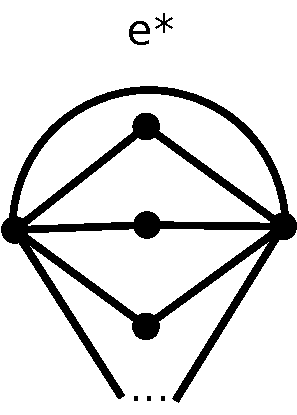
\includegraphics[width=2cm]{files/c2nex1.pdf}}
\end{center}

Nous appelons cette arrête spéciale $e^*$. Nous avons donc :
\[ C_{2,n}-e^* = K_{2,n} \]
et
\[ C_{2,n} \backslash{e^*} = S_{n-1} \]
Nous rappelons que $S_n$ est un arbre. Finalement nous admettrons :
\[ \forall{e} \hspace{3mm} K_{2,n}-e = K_{2,n}(k-1) \]
En effet il ne reste que $K_{2,n-1}$ plus un sommet pendant, donc coloriable de $k-1$ manières :

\begin{center}
$K_{2,n-1}^{+1}$ : \raisebox{-0.5\height}{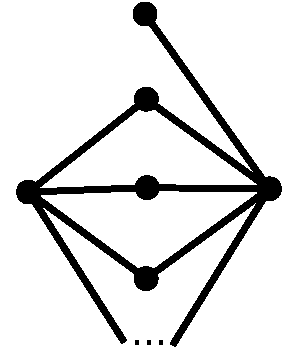
\includegraphics[width=2cm]{files/k2n_dangle_ex1.pdf}}
\end{center}

Supposons alors $H(n)$ vrai pour un $n$ donnée. 
\begin{eqnarray*}
P_{K_{2,n+1}}(k)			& = & P_{K_{2,n+1}-e} - P_{K_{2,n+1} \backslash{e}}				\\
							& = & P_{K_{2,n}}(k-1) - P_{C_{2,n}}							\\
							& = & P_{K_{2,n}}(k-1) - P_{K_{2,n}} + P_{S_{n-1}}					\\
							& = & (k-2)\big(k(k-1)^n + k(k-1)(k-2)^n\big) + k(k-1)^{n-2}	\\
							& = & \ldots													\\
							& = & k(k-1)^{n+1} + k(k-1)(k-2)^{n+1}
\end{eqnarray*}
Nous avons donc $H(n+1)$.
\end{itemize}
Comme $H(1) \wedge (H(n) \Rightarrow H(n+1))$, alors par récurrence $H(n)$ sera vrai pour tout $n \geq 1$.
